\documentclass[9pt]{beamer}
%\usetheme{Malmoe}
\usetheme{Darmstadt}
\usecolortheme{beaver}
\setbeamertemplate{navigation symbols}{}
\beamersetuncovermixins{\opaqueness<1>{25}}{\opaqueness<2->{15}}
\usepackage{url}
\usepackage{ragged2e}
\usepackage{multirow}
\usepackage{minted}
%\usepackage{color}
\usepackage{subfigure}
%\usepackage[square,sort&compress]{natbib} 
\usepackage{graphics}
\usepackage{epsfig}
\usepackage{times}
\usepackage{amsmath}
\usepackage{amssymb}
\usepackage{color}
\usepackage{algorithm}
\usepackage{algorithmic}
\usepackage{multirow}
\def\imagetop#1{\vtop{\null\hbox{#1}}}

\definecolor{blue}{rgb}{.1,.1,.5}
\definecolor{lightblue}{rgb}{.1,.1,.9}
\definecolor{darkred}{rgb}{.7,.1,.1}
\definecolor{bg}{rgb}{.9,.9,.1}
\def\slantfrac#1#2{\kern.1em^{#1}\kern-.3em/\kern-.1em_{#2}}

\logo{
\includegraphics[width=1in]{pics/UdeM_NoirBleu_logo_Marie_crop.pdf}}
% Standard LaTeX stuff - note the optional abbreviated title being provided
\title[Theano Tutorial]{Introduction to Theano}
\author[Razvan Pascanu]{Razvan Pascanu\\ Professeur: Yoshua Bengio}

\date{\today}

\setbeamertemplate{footline}{\hspace*{.5cm}\scriptsize{Razvan Pascanu  ---
Theano Tutorial
\hspace*{50pt} \hfill\insertframenumber\hspace*{.5cm}}} 
\renewcommand{\theFancyVerbLine}{\sffamily
\textcolor[rgb]{0.5,0.5,1.0}{\scriptsize
\oldstylenums{\arabic{FancyVerbLine}}}}

\begin{document}


\frame{\titlepage}

\section*{Outline}
\begin{frame}
    %\frametitle{Outline}
    \begin{columns}[b]
    \column{.6\textwidth}
        \begin{itemize}
            \item The Tools
            \begin{itemize}
                \item Git and Assembla
                \item How to install Theano
                \item The list of tools
            \end{itemize}
            \item Theano
            \begin{itemize}
                \item Theano at a Glance
                \item Numpy refresher
                \item Adding two numbers
                \item Computing derivatives
                \item Shared variables
                \item Details of theano.function
                \item Basic debugging
                \item Basic profiling
            \end{itemize}
            \item Deep Learning Tutorials
            \begin{itemize}
                \item Putting it all together: Logistic Regression
            \end{itemize}
            \item Q\&A
        \end{itemize}
    \column{.4\textwidth}
        
\includegraphics[width=.6\textwidth]{pics/lisabook_logo_text2.png} 
    \end{columns}
\end{frame}

\section{The Tools}
\subsection{Git and Assembla}
\begin{frame}
    %\frametitle{Git and Assmebla}
        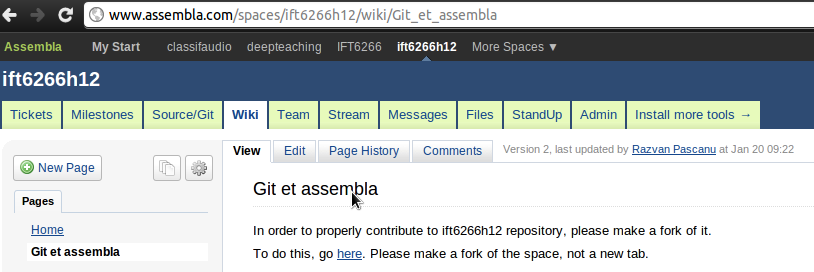
\includegraphics[width=.8\textwidth]{pics/assembla.png} 
    \begin{itemize}
        \item Repo: \url{http://www.assembla.com/spaces/ift6266h12/wiki}
    \end{itemize}
    {\color{darkred}TODO}:
    \begin{itemize}
        \item Make an assembla account
        \item Join the team (you can send me the username at \url{pascanur@iro.umontreal.ca})
        \item Create a fork of the repository
        \item Learn to properly use {\color{darkred} Git}
    \end{itemize}
\end{frame}

\subsection{Installing Theano}
\begin{frame}
    %\frametitle{Installing Theano}
    \begin{center}
    {\Huge \emph{RTFM}}
    \end{center}

    \url{http://deeplearning.net/software/theano/install.html}
\end{frame}

\subsection{List of tools}
\begin{frame}
    %\frametitle{List of tools}
    \begin{itemize}
        \item Mandatory
        \begin{itemize}
            \item Assembla [\url{www.assembla.com}]
            \item Git [\url{www.git-scm.com}]
            \item jobman, jobdispatch [\url{www.deeplearning.net/software/jobman}]
            \item NumPy [\url{www.numpy.org}]
            \item python [\url{www.python.org}]
            \item psql [\url{http://www.postgresql.org}]
            \item SciPy [\url{www.scipy.org}]
            \item Theano [\url{www.deeplearning.net/software/theano}]
        \end{itemize}
        \item Optional
        \begin{itemize}
            \item ipdb [\url{pypi.python.org/pypi/ipdb}]
            \item IPython [\url{www.ipython.org}]
            \item matplotlib [\url{http://matplotlib.sourceforge.net/}]
        \end{itemize}
    \end{itemize}
\end{frame}

\section{Theano}
\subsection{Theano at a Glance}

\begin{frame}[fragile]
    \definecolor{bg}{rgb}{.9,.9,.9}
    \begin{minted}[linenos=True, bgcolor=bg, frame=lines, mathescape=True]{python}
        # Compute $\sum_{i=0}^N x_i^2$
        import theano, theano.tensor as TT
        x = TT.vector()
        rval = (x ** 2).sum()
        fn = theano.function([x], rval, 
                    allow_input_downcast = True)

        assert 14 == fn([1, 2, 3])

    \end{minted}
    \begin{itemize}
        \item execution speed optimization
        \item symbolic differentiation
        \item stability optimization
    \end{itemize}
\end{frame}
\subsection{Numpy refresher}
\begin{frame}[fragile]
    \begin{itemize}
        \item The fundamental package for scientific computing in Python
        \item Linear algebra (and more) on multidimensional tensors
        \item Random number generators 
        \item and much, much more
        \item all in the friendly python syntax
    \end{itemize}
    \bigskip
    \definecolor{bg}{rgb}{.9,.9,.9}
    \begin{minted}[linenos=True, bgcolor=bg, frame=lines, mathescape=True]{python}
        import numpy
        W = numpy.random.uniform(size=(3,3))
        X = numpy.asarray([1,0,1])
        print numpy.dot(W,X)
    \end{minted}

    See ipython notebook example.
\end{frame}
\subsection{Theano basics}
\begin{frame}
    Is as simple as following these simple steps:
    \begin{enumerate}
        \item Declare {\it variables}, specifying the types
        \item Write down the expression in terms of the variables
        \item {\it Compile the function} that will compute the expression
        \item Call the function on the intended data 
    \end{enumerate}
    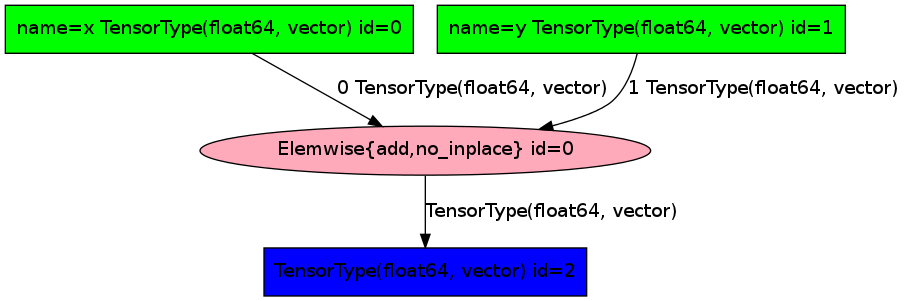
\includegraphics[width=.8\textwidth]{pics/compgraph1.png} 
    \bigskip
    \begin{center}
    See ipython notebook example.
    \end{center}
\end{frame}
\subsection{Computing derivatives}
\begin{frame}[fragile]
    \begin{itemize}
    \item Theano provides symbolic differentiation 
    \item The computational graph representing the gradients is
    automatically optimized
    \item And all this at a single call away: \texttt{TT.grad(cost, wrt)}
    \end{itemize}

    \begin{minted}[linenos=True, bgcolor=bg, frame=lines, mathescape=True]{python}
        import theano, theano.tensor as TT
        x = TT.vector('x')
        rval = TT.tanh(x ** 2)
        fn_forward = theano.function([x], rval)
        gx = TT.grad(rval, x)
        fn_grad = theano.function([x], gx)
    \end{minted}
\end{frame}
\begin{frame}
    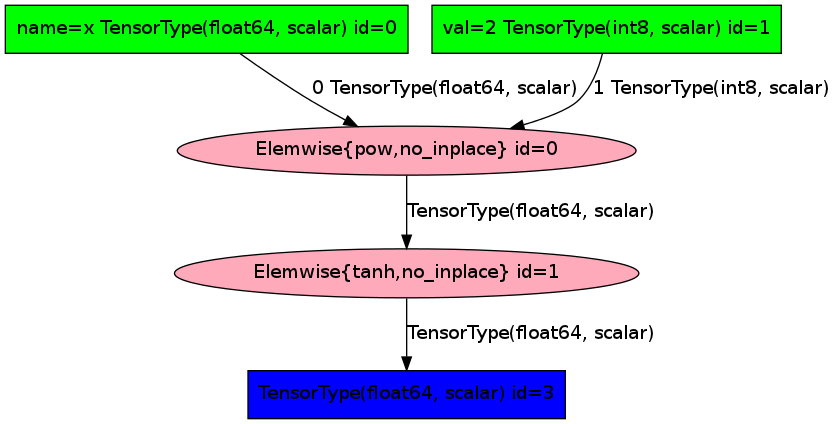
\includegraphics[width=.8\textwidth]{pics/compgraph2.png}
    
    \begin{equation}
        \frac{\partial \tanh(x^2)}{\partial x} = \frac{\partial \tanh(x^2)}{\partial x^2} \frac{\partial x^2}{\partial x} =  
         \frac{\partial \tanh(x^2)}{\partial \tanh(x^2)}\frac{\partial \tanh(x^2)}{\partial x^2} \frac{\partial x^2}{\partial x} 
    \end{equation}

\end{frame}
\begin{frame}
    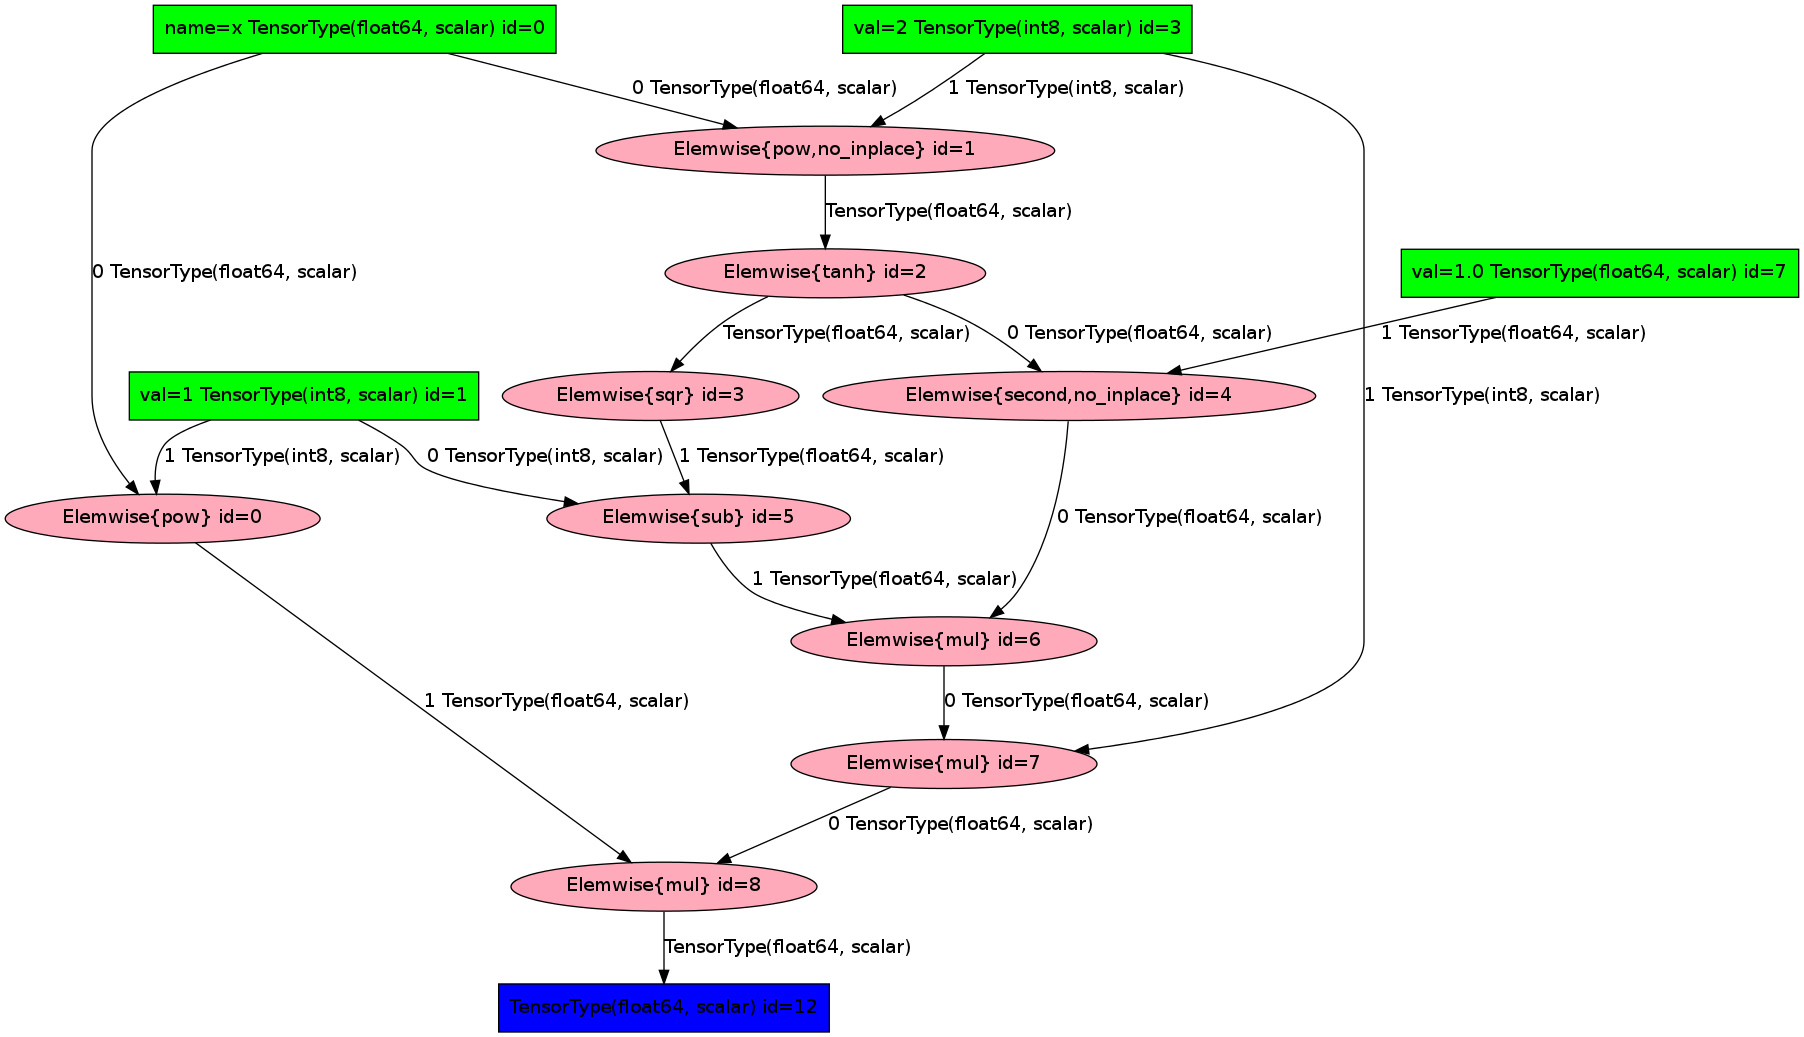
\includegraphics[width=1\textwidth]{pics/compgraph3.png} 

\end{frame}

\subsection{Shared variables}
\begin{frame}
    \begin{itemize}
        \item Think of them as global variables
        \item They have a state that stays consistent in between calls
        \item Especially useful to keep memory on the same device 
        \item Can be updated via \texttt{set\_value} and \texttt{updates} provided 
        to \texttt{theano.function}
    \end{itemize}
    \bigskip
    See ipython notebook example.
\end{frame}
\subsection{Details of theano.function}
\begin{frame}[fragile]

    \definecolor{bg}{rgb}{.9,.9,.9}
    \begin{minted}[linenos=True, bgcolor=bg, frame=lines, mathescape=True]{python}
        def function(inputs, 
                     outputs=None, 
                     mode=None, 
                     updates=[], 
                     givens=[],
                     no_default_updates=False, 
                     accept_inplace=False, 
                     name=None,
                     rebuild_strict=True, 
                     allow_input_downcast=None, 
                     profile=None):
    \end{minted}
\end{frame}
\subsection{Basic debugging}
\begin{frame}
    \begin{itemize}
        \item Use {\bf test values}
        \item Use \texttt{theano.printing.Print} to print intermediate results
        \item Use \texttt{theano.printing.pydotprint} to visualize the
                computational graph
        \item Run in \texttt{DEBUG\_MODE}
    \end{itemize}
    \bigskip
    \begin{center}
    See ipython notebook example.
    \end{center}
\end{frame}
\subsection{Basic profiling}
\begin{frame}
    \begin{center}
    See ipython notebook example.
    \end{center}
\end{frame}
\section{Deep Learning Tutorials}
\subsection{Logistic Regression}
\begin{frame}
    \url{http://deeplearning.net/tutorial/logreg.html\#logreg}
\end{frame}
\section{Questions}
\begin{frame}
    \begin{center}
    {\Huge Questions ? }
    \end{center}
\end{frame}
\end{document}
